\documentclass[]{report}

\usepackage{hyperref}
\usepackage{float}
\usepackage{needspace}
\usepackage{interval}
\usepackage{pgfplots}
\usepackage{neuralnetwork}
\usepackage[utf8]{inputenc}
\usepackage[T1]{fontenc}
\usepackage[a4paper, left=2.5cm, right=2.5cm, top=2cm, bottom=2cm]{geometry}

\hypersetup{
    colorlinks=true,
    linkcolor=blue,
    filecolor=magenta,      
    urlcolor=black,
}

\renewcommand{\thesection}{\Alph{section}}
\renewcommand{\thesubsection}{\arabic{subsection}}
\renewcommand{\thesubsubsection}{(\emph{\alph{subsubsection}})}

\title{The math behind an artificial neural network}
\author{Hugo Lageneste}
\date{January 2020}

\begin{document}

\begingroup
\let\cleardoublepage\relax
\let\clearpage\relax

\tableofcontents

\needspace{6cm}
\[\;\]

\vfill

\endgroup

\chapter*{The math behind an artificial neural network}

\setcounter{section}{-1}
\section{Introduction}

\subsection{Application example}

{Let's take an example to see how an ANN\footnote{Artificial Neural Network} works.}

\begin{figure}[H]
    \centering
    \begin{tabular}{|l|c|c|r|}
      \hline
      Obesity & Exercise & Smoking & Diabetic \\
      \hline
      1 & 0 & 0 & 1 \\
      0 & 1 & 0 & 0 \\
      0 & 0 & 1 & 0 \\
      1 & 1 & 0 & 1 \\
      \hline
    \end{tabular}
    \caption{Example of a set of persons with Obesity, Exercise, Smoking and Diabetic characteristics}
\end{figure}

{In the precedent figure, the 1 stands for true and the 0 for false. We can observe that in this example, a person with diabetes is inevitably obese. What if we want a program which takes only in parameter those 4 examples and can predict with different examples if a person is diabetic or not?}\\

{We can model this program as an ANN with 3 input neurons which represent the Obesity, Exercise and Smoking columns and a single output neuron which represents
the Diabetic column.}

\begin{figure}[H]
    \centering
    \begin{neuralnetwork}[height=3, nodespacing=15mm]
        \inputlayer[count=3, bias=false, title=Input layer]
        \outputlayer[count=1, title=Output layer]
        \linklayers
    \end{neuralnetwork}
    \caption{Diagram of the ANN to model the example}
\end{figure}

\subsection{Neural network operation}
\label{subsec:operation}

{The input values will be inserted in the input neurons and the network will operate as a “function” to say if the person is diabetic or not. Each liaison between each neuron is a value called weight and
is unique. And each neuron holds a specific value, calculated with the previous neuron values and the
weights. The whole goal of the neural network is to find the correct weights to make the final predictions
right.}\\

{To make the weights right, we will proceed in different steps. First of all, the neural network will
compute the value of the output layer’s neurons named the prediction. Then, the network will make
the difference between the prediction and the actual output and will adjust the weights to make the
prediction more accurate. This process will be repeated until the success rate is convenient.}\\

{After the construction of the neural network, we will be able to send values like 1, 1 and 1 (so it means that the persons is obese, does exercise and smokes) and get an answer from the neural network which tells us that the person is diabetic.}



\section{Forward propagation}

{As seen in the Introduction, each neuron holds a value contained between 0 and 1, calculated with the values of the previous neurons, the weights and a bias. We are going to see how these values are calculated.}

\begin{figure}[H]
    \centering
    \begin{neuralnetwork}[height=4, nodespacing=15mm]
        \newcommand{\inputtext}[2]{$a^{(l-1)}_#2$}
        \newcommand{\outputtext}[2]{$a^{(l)}_#2$}
        \inputlayer[count=3, bias=false, text=\inputtext, title=Input layer]
        \outputlayer[count=1,  text=\outputtext, title=Output layer]
        \linklayers[title=Weights $w_k$]
    \end{neuralnetwork}
    \caption{Diagram of a neural network, the exponent represents the index of the layer and the subscript the index of the neuron then $a$ is the value held in the neuron.}
\end{figure}

{Let's create a notation, $z^{(l)}_1$ which is the bias added to the dot product of weights $w_k$ and values of the previous neurons $a^{(l-1)}_k$.}

\[{z^{(l)}_1=b^{(l)}_1+\sum_{k=1}^{n_{(l-1)}} a^{(l-1)}_k w_k}\]

{In order to keep the values in the neurons between 0 and 1, we are going to use the sigmoid function which is defined on $\interval[open]{0}{1}$, noted :}
\[\sigma(x)=\frac{1}{1+e^{-x}}\]

\begin{figure}[H]
    \centering
    \begin{tikzpicture}
        \begin{axis}[grid=major, xmax=6, ymax=1.1, samples=50, xlabel=$x$, ylabel=$\sigma(x)$]
          \addplot[black, thin] (x,1/(1+e^(-x)));
        \end{axis}
    \end{tikzpicture}
    \caption{Graphical representation of the sigmoid function}
\end{figure}

{Thus,}

\[a^{(l)}_1=\sigma\left(z^{(l)}_1\right)\]
\[a^{(l)}_1 \in \interval[open]{0}{1}\]

{This calculus can be too visualised with matrix}

\[a^{(l)}_1=\sigma\left(\begin{bmatrix}w_1 & w_2 & w_3\end{bmatrix}\begin{bmatrix}a^{(l-1)}_1 \\ a^{(l-1)}_2 \\ a^{(l-1)}_3\end{bmatrix}+\begin{bmatrix}b^{(l)}_1\end{bmatrix}\right)\]

\section{Back propagation}

\subsection{Cost function}

{Let's take a simple example of a one-input-layer-one-output-layer-neural-network}

\begin{figure}[H]
    \centering
    \begin{neuralnetwork}[height=2, nodespacing=15mm]
        \newcommand{\inputtext}[2]{$a^{(l-1)}$}
        \newcommand{\outputtext}[2]{$a^{(l)}$}
        \inputlayer[count=1, bias=false, text=\inputtext, title=Input layer]
        \outputlayer[count=1,  text=\outputtext, title=Output layer]
        \linklayers[title=Weight $w$]
    \end{neuralnetwork}
    \caption{Diagram of the ANN to model the example of the cost function}
    \label{fig:simplenn}
\end{figure}

{Once again,}

\[z^{(l)}=b+a^{(l-1)}w\]
\[a^{(l)}=\sigma\left(z^{(l)}\right)\]

{The goal is now to adjust the weights to make the prediction more accurate. Let's introduce the cost function which calculates the square difference between the prediction and the actual output $y$.}

\[C_1\left(a^{(l)},y\right)=\left(a^{(l)}-y\right)^2\]

{The smaller the cost function is, the more accurate the predictions are, mathematically the goal is to minimize the cost function.}

\begin{figure}[H]
    \centering
    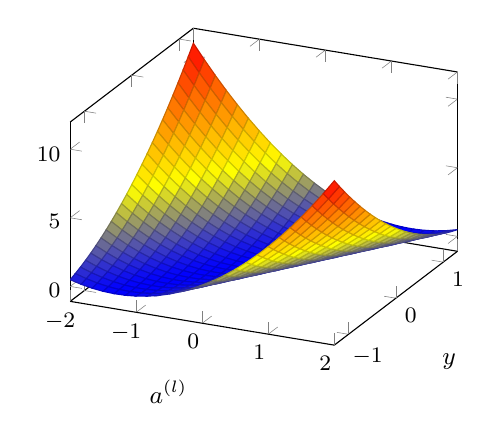
\begin{tikzpicture}
        \begin{axis}[
            xlabel=$a^{(l)}$, ylabel=$y$,
        	small,
        ]
        \addplot3[
        	surf,
        	domain=-2:2,
        	domain y=-1.3:1.3,
        ] 
        	{(x-y)^2};
        \end{axis}
    \end{tikzpicture}
    \caption{Cost function graphical representation of the neural network, figure \ref{fig:simplenn}}
\end{figure}

\subsection{Gradient descent}

{Now we will need to understand how sensitive the cost function is to small changes to $w_k$ because remember from \ref{subsec:operation}, the goal is to adjust weights. Thus, we will determine the partial derivative of $C$ with respect to $w$ using the chain rule.}

\[{\frac{\partial C_1}{\partial w}=\frac{\partial C_1}{\partial a^{(l)}} \frac{\partial a^{(l)}}{\partial z^{(l)}} \frac{\partial  z^{(l)}}{\partial w}}\]

{Indeed,}

\[\frac{\partial C_1}{\partial a^{(l)}}=2\left(a^{(l)}-y\right)\]
\[\frac{\partial a^{(l)}}{\partial z^{(l)}}=\frac{\partial \sigma\left(z^{(l)}\right)}{\partial z^{(l)}}=\sigma\prime\left(z^{(l)}\right)\]
\[\frac{\partial  z^{(l)}}{\partial w}=\frac{\partial  \left(b+a^{(l-1)}w\right)}{\partial w}=a^{(l-1)}\]

{All together, it gives us}

\[\frac{\partial C_1}{\partial w}=2\left(a^{(l)}-y\right) \sigma\prime\left(z^{(l)}\right) a^{(l-1)}\]

{We will use this formula to calculate the adjustments to make to the weights multiple times until the predictions are accurate.}

\[w=w+\alpha \frac{\partial C_1}{\partial w}\]

\section{Complex example}

\begin{figure}[H]
    \centering
    \begin{neuralnetwork}[height=5, nodespacing=15mm]
        \newcommand{\inputtext}[2]{$a^{(l-2)}_#2$}
        \newcommand{\hiddentext}[2]{$a^{(l-1)}_#2$}
        \newcommand{\outputtext}[2]{$a^{(l)}_#2$}
        \inputlayer[count=3, bias=false, text=\inputtext, title=Input layer $a^{(l-1)}_k$]
        \hiddenlayer[count=4, bias=false, text=\hiddentext]
        \linklayers[title={Weights $w^{(l-1)}_{jk}$}]
        \outputlayer[count=1,  text=\outputtext, title=Output layer $a^{(l)}_j$]
        \linklayers[title={Weights $w^{(l)}_{jk}$}]
    \end{neuralnetwork}
    \caption{Diagram of a more complex ANN}
\end{figure}

{We will model this problem with matrices.}

\subsection{Forward propagation}

{First of all we are going to create a matrix for each weights' layer}

\[w^{(l-2)}=\begin{bmatrix}
w_{11} & w_{12} & w_{13} & w_{14}\\
w_{21} & w_{22} & w_{23} & w_{24}\\
w_{31} & w_{32} & w_{33} & w_{34}\\
\end{bmatrix}\]

\[w^{(l-1)}=\begin{bmatrix}
w_{11}\\
w_{21}\\
w_{31}\\
w_{41}\\
\end{bmatrix}\]

{A layer is represented by a $t$ by $k^{(l)}$ Matrix, where $t$ is the number of training examples and $k$ the number of nodes in a layer}

\[a^{(l-2)}=\begin{bmatrix}
a^{(l-2)}_1 & a^{(l-2)}_2 & a^{(l-2)}_3 \\
\end{bmatrix}\]

{Then, to calculate the next layer's values we need to express $z$ to compute $a$.}

\[z^{(l)}=a^{(l-1)} \cdot w^{(l)}+b^{(l-1)}\]
\[a=\sigma (z)\]

\subsection{Back propagation}
{Because we have now a hidden layer, we will need to express the partial derivative of $C$ with respect to $w^{(l)}$ couched in terms of $l$.}\\
{The adjustments will take the following form}
\[w^{(l)}=w^{(l)}+\alpha \frac{\partial C}{\partial w^{(l)}}\]
{Here, $\alpha$ represents the learning rate.}\\
{Thus, we need to compute this derivative $\frac{\partial C}{\partial w^{(l)}}$.}
{Using the chain rule,}
\[\frac{\partial C}{\partial w^{(l)}}=\frac{\partial C}{\partial z^{(l)}} \frac{\partial z^{(l)}}{\partial w^{(l)}}\]
{First of all let's compute $\frac{\partial z^{(l)}}{\partial w^{(l)}}$}
\[\frac{\partial z^{(l)}}{\partial w^{(l)}} = \frac{\partial}{\partial w^{(l)}} \left( a^{(l-1)} w^{(l)} + b^{(l-1)} \right)=a^{(l-1)}\]
{Then, we'll compute $\frac{\partial C}{\partial z^{(l)}}$ couched in terms of $z^{(l+1)}$ in order to model backpropagation in programming.}
\[\frac{\partial C}{\partial z^{(l)}}=\frac{\partial C}{\partial z^{(l+1)}}\frac{\partial z^{(l+1)}}{\partial a^{(l)}}\frac{\partial a^{(l)}}{\partial z^{(l)}}\]
\[\frac{\partial z^{(l+1)}}{\partial a^{(l)}}=\frac{\partial}{\partial a^{(l)}} \left(w^{(l+1)} a^{(l)} + b^{(l)}\right)=w^{(l+1)}\]
\[\frac{\partial a^{(l)}}{\partial z^{(l)}}=\frac{\partial}{\partial z^{(l)}} \sigma \left(z^{(l)}\right)=\sigma\prime\left(z^{(l)}\right)\]
{Thus, after adjusting the terms to make dot products working we got}
\[\frac{\partial C}{\partial z^{(l)}}=\left(w^{(l+1)^{T}} \cdot \frac{\partial C}{\partial z^{(l+1)}} \right) \times \sigma\prime\left(z^{(l)}\right)\]
{And,}
\[\frac{\partial C}{\partial w^{(l)}}=\left(w^{(l+1)^{T}} \cdot \frac{\partial C}{\partial z^{(l+1)}} \right) \times \sigma\prime\left(z^{(l)}\right) \times a^{(l-1)}\]
{As you can see here, to compute the adjustments for the weights you need the derivative of $C$ with respect to the next $z$ so we will need to calculate the derivative of $C$ with respect to $z$ for the last layer so we never run get out of the range.}
{Here $L$ is the last layer}
\[\frac{\partial C}{\partial z^{(L)}}=2(a^{(L)}-y) \sigma\prime\left(z^{(L)}\right)\]
\[\frac{\partial C}{\partial z^{(L)}}=2(a^{(L)}-y)\sigma\left(z^{(L)}\right)\left(1-\sigma\left(z^{(L)}\right)\right)\]
\[\frac{\partial C}{\partial z^{(L)}}=2(a^{(L)}-y)a^{(L)}\left(1-a^{(L)}\right)\]
{Here we have all the ressources we need to build an artificial neural network.}

\end{document}